\documentclass{ecai}
\usepackage{times}
\usepackage{graphicx}
\usepackage{latexsym}
\usepackage{xspace}
\usepackage{hyperref}
\usepackage{algorithm}
\usepackage[noend]{algpseudocode}
\usepackage[numbers]{natbib}
\usepackage{notoccite}

\usepackage[dvipsnames]{xcolor}
\newcommand{\sergey}[1]{\textcolor{magenta}{{\sc Sergey:} #1}\xspace}
\newcommand{\samuel}[1]{\textcolor{green}{{\sc Samuel:} #1}\xspace}

%%\ecaisubmission   % inserts page numbers. Use only for submission of paper.
                  % Do NOT use for camera-ready version of paper.

\begin{document}

\title{Tabular Constraint Learning}

\author{Name1 Surname1 \and Name2 Surname2 \and Name3 Surname3 \institute{KU Leuven, Belgium, email: firstname.lastname@kuleuven} }

\maketitle

\begin{abstract}
  abstract
\end{abstract}
\section{Introduction}
\sergey{bullet points for luc to start introduction}\\
\textbf{Key question}:\\
Can we discover or reconstruct structural relations in flat tabular spreadsheet data? [in a general way that allows declarative specification of constraints to discover]\\


\textbf{Motivation}:
\begin{itemize}
  \item File generated from model, model got lost, need to reconstruct
  \item Constraint programming is hard - is Excel hard?
  \item Avoid manual analysis, provide selection of constraints
  \item Error checking
  \item Completion, gain speed and insights (Complicated constraints, also complicated to verify, too much output)
\end{itemize}

\textbf{Novelty:}
\begin{itemize}
  \item Unsupervised setting (contrary to flashfill, etc)
  \item Numeric, different constraints (contrary to single textual function solution in flashfill, etc)
  \item Data format (2D) -- data is no longer in rows like a classic ML or DM settings
  \item Declarative, general / modular, stacking of constraint problems 
\end{itemize}

\sergey{to himself we need structure here} 
\begin{figure}[thpb]
  \begin{center}
    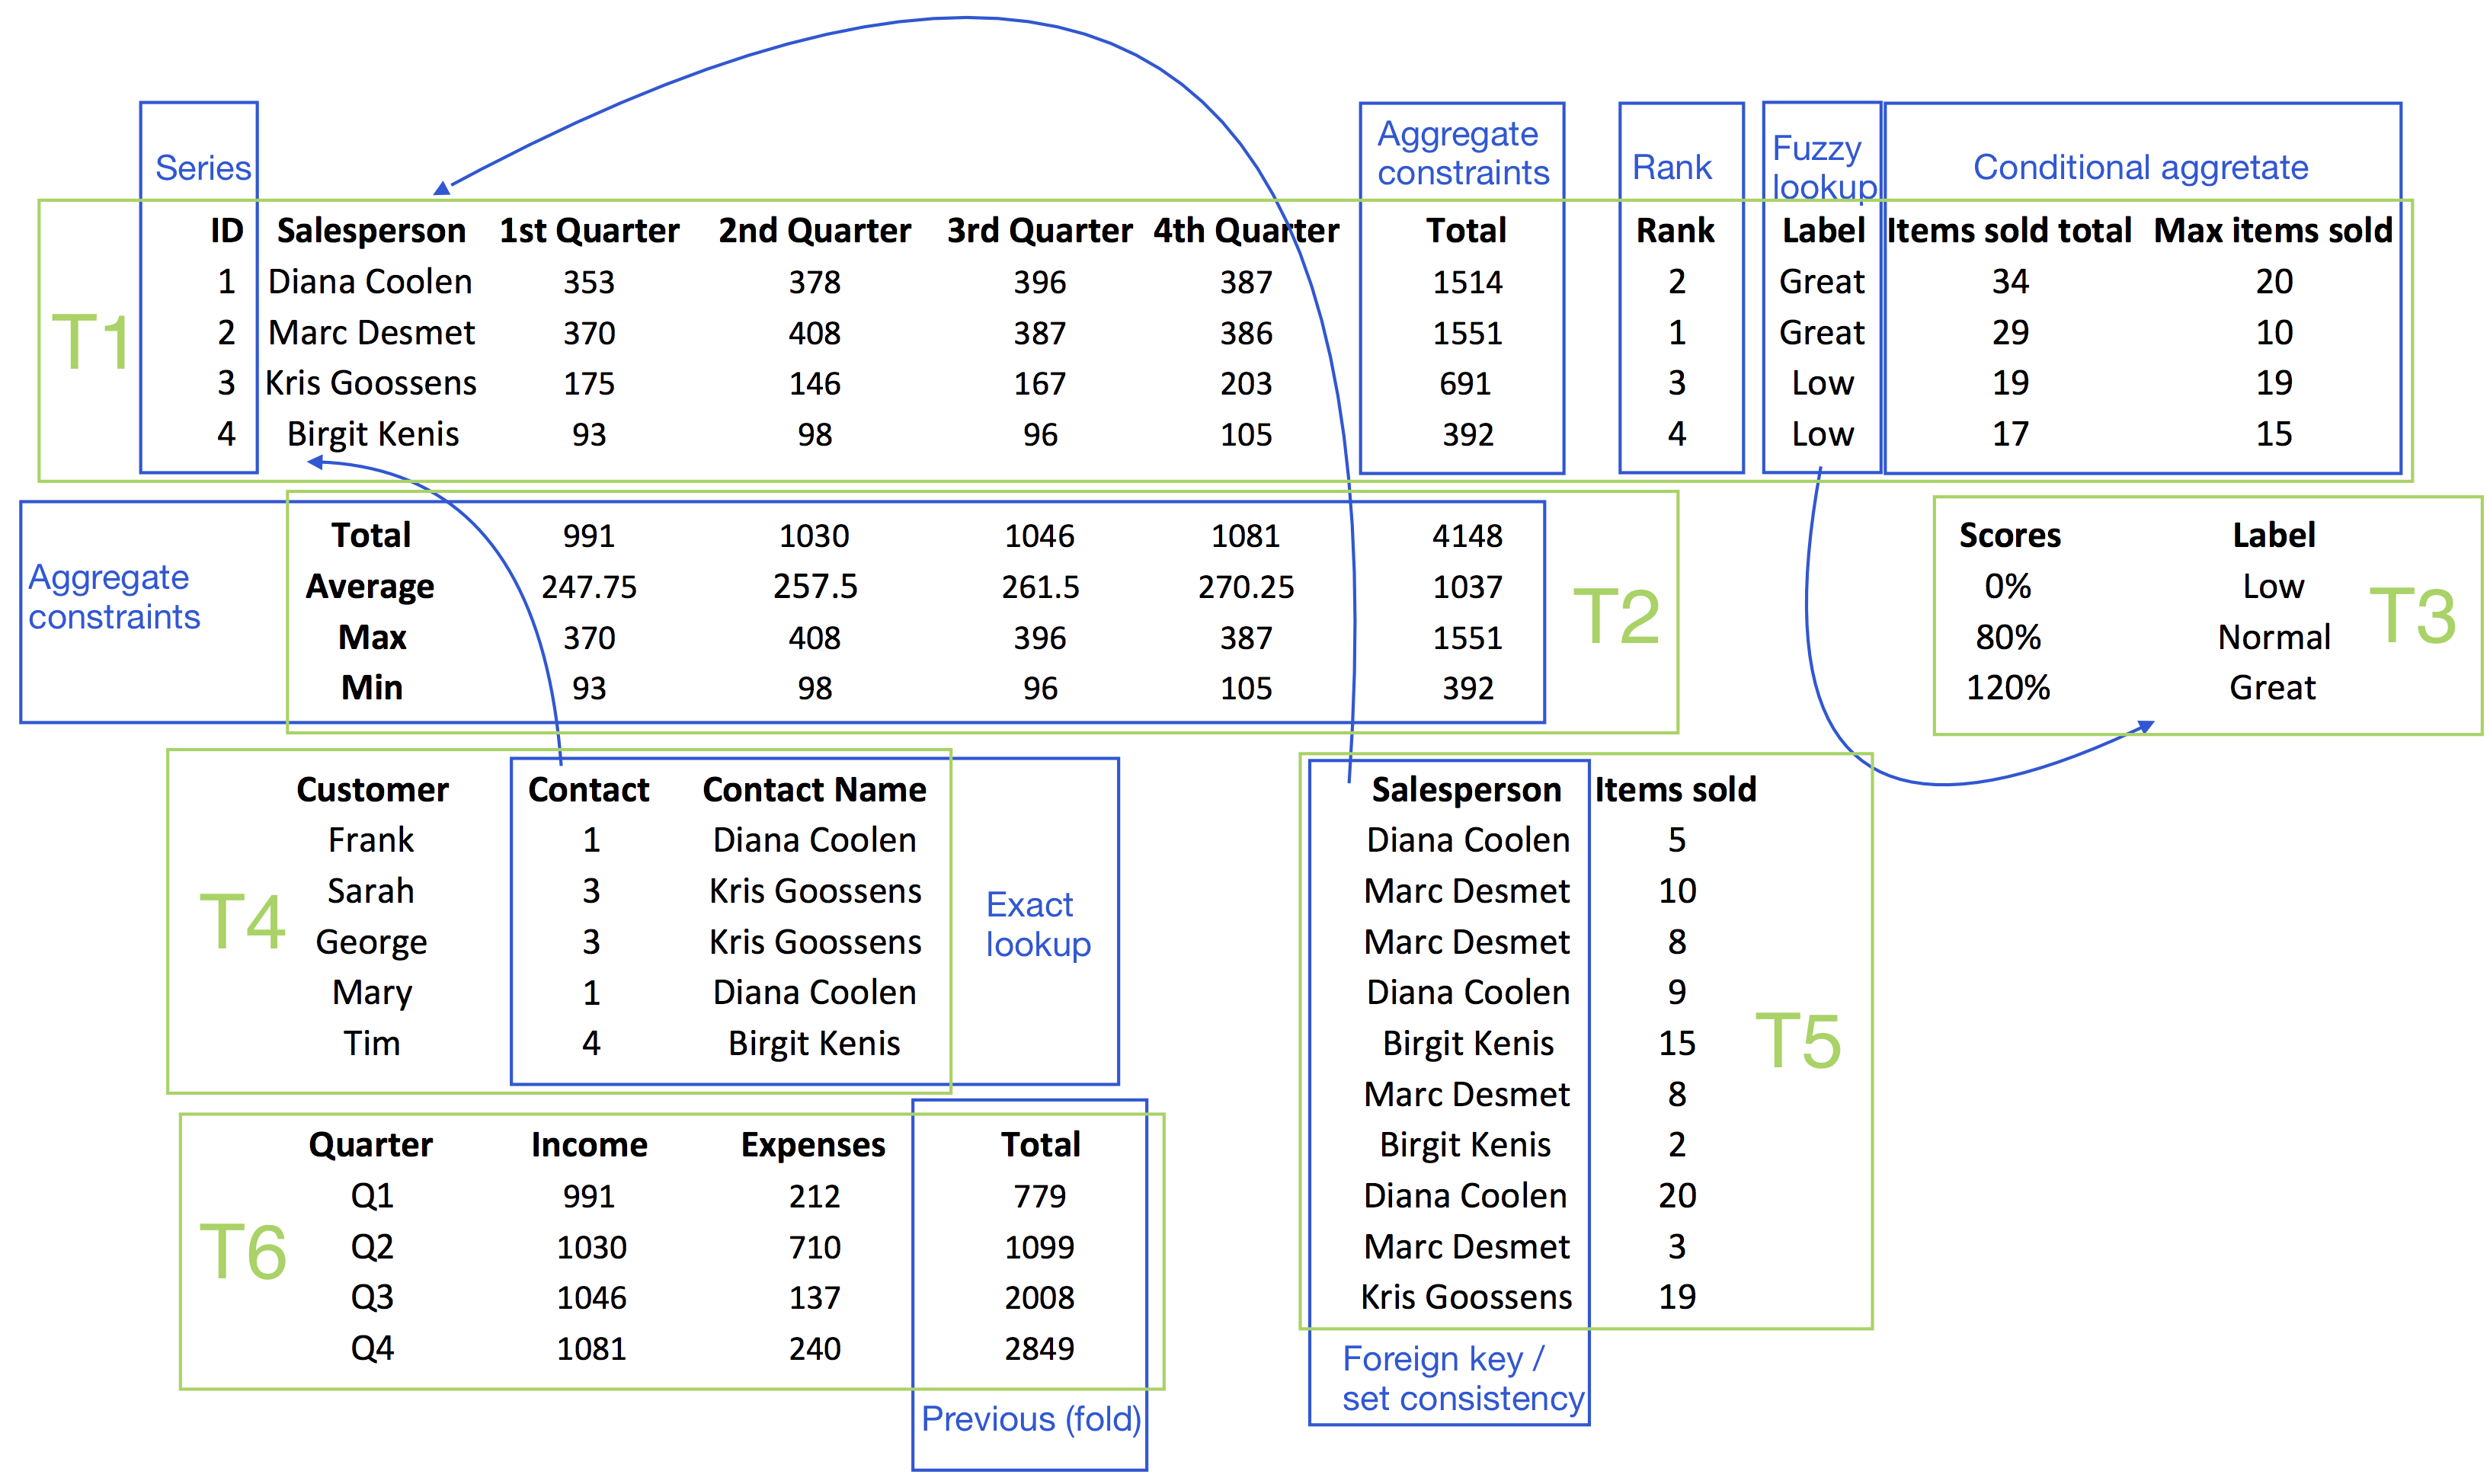
\includegraphics[width=0.51\textwidth]{figures/Demo.png}
  \end{center}
  \vspace{-10pt}
  \caption{An example of constraint reconstruction (in blue) with indicated groups (in green)}
  \label{fig:main_example}
\end{figure}

\section{Formalization}

\newcommand{\constraints}{\ensuremath{\mathcal{C}}\xspace}
\newcommand{\format}[1]{\textit{#1}\xspace}
\newcommand{\generategroups}{\format{generateAssignments}}
\newcommand{\extractgroups}{\format{extractGroups}}
\newcommand{\extracttables}{\format{extractTables}}
\newcommand{\learnconstraints}{\format{learnConstraints}}
\newcommand{\findassignment}{\format{findSolutions}}
\newcommand{\postprocess}{\format{pruneRedundant}}

\newcommand{\CName}{Name\xspace}
\newcommand{\CSignature}{Signature\xspace}
\newcommand{\CFunction}{Function\xspace}

\begin{algorithm}[thb]
  \begin{algorithmic}
    \footnotesize
    \State \textbf{Input:} $G$ -- set of groups
    \State \textbf{Output:} $S$ -- learned constraints with their satisfaction assignments
    \State $S \gets \emptyset$ \Comment{The set of solutions}
  \For{$c \in \constraints$} \Comment{\constraints -- partially ordered set of Excel constraints; Table \ref{table:constraints}}
  \State $v_1, ..., v_n =$ variables of $c$ 
    \For{$v_1{:}~G_1, \dots, v_n{:}~G_n \in \generategroups(c, G, S)$}
      \State $S \gets S \cup \findassignment(c, v_1{:}~G_1, \dots, v_n{:}~G_n, S)$
    \EndFor
  \EndFor\\
\Return $S$
\end{algorithmic}
\caption{Tabular constraint learning}
\label{algo:tcl}
\end{algorithm}
\subsection{Groups, Type-consistency and Constraints}
In this work we distinguish the following types of data: numeric and textual. The numeric type has two subtypes: integers and floats. We also consider the special element called \textit{None}, which has two types: numeric and textual. A set is called \textit{type-consistent} iff all elements are either numeric or textual. Certain constraints, such as \textit{rank} or \textit{series}, make use of the numeric sub-types by requiring its arguments to be integers.

A \textit{vector} is a subrange of a column or of a row that is type-consistent. If a vector is a subrange of a row (column), we say that it has a \textit{row} (\textit{column}) orientation. A \textit{group} is a subrange of vectors with the same orientation in a table. We use the following notation to refer to a row group $G$ in the $N$-th table with rows ranging from $a$ to $b$: $G = T_N[a{:}b,:]$, where $N,a,b$ are natural numbers. Similarly for a column group $G$ ranging from $a$ to $b$ columns in the $N$-th table we write $G = T_N[{:},a{:}b]$.

A \textit{constraint} is a triple of \textit{(\CName,\CSignature,\CFunction)}, where \CName is a textual name of the constraint; \CSignature is the signature of the constraint consisting of its arity and properties of the arguments, such as their types, sizes (properties might constrain sizes of two arguments as well, by for example, require them to be equal), etc; \CFunction is the function over arguments specified in \CSignature that represents constraint satisfaction. For example, a column-wise sum constraint has \CName equal to \textit{Y = SUM(X, col)}, its \CFunction sets arity to 2 and both arguments must be numeric and \sergey{Samuel, could you put the actual properties and \CFunction here?}

\subsection{Constraint learning algorithm description}
Let us describe the key steps and functions in Algorithm \ref{algo:tcl}. Essentially, the algorithm has two steps: candidate group generation and subgroup satisfaction search, which is in line with the well-known in AI paradigm of ``generate-and-test'' \cite{whaisasp}. Let us elaborate on each step in detail.

\paragraph{Candidate group generation} $\generategroups(\textit{Constraint,GroupSet,Solutions})$ is the function generating tuples of groups that are legitimate solution candidates e.g., $X,Y$ are variables of \textit{Y = SUM(X)} and $X,Y$ satisfy the following constraints \sergey{Samuel, can you add here, what is actually used for the sum now?}. Essentially, the group generation step is a constraint satisfaction problem associated with the specific constraint. However, many constraints have the same candidate generation procedures, e.g., min, max, avg, count, etc.

\paragraph{Subgroup satisfaction search} $\findassignment(\textit{Constraint,Candidates,Solutions})$ is the function looking for the subsets of vectors in the candidates satisfying the constraint. If multiple subsets satisfy the constraint, a maximal is selected. If $G_1,G_2$, associated with the variables $X,Y$ in the constraint \textit{Y = SUM(X)}, are candidates, then \findassignment selects a single vector $y$ in $G_2$ and consecutive subset of vectors $x$ in $G_1$ such that the sum over $x$ is equal to $y$. For example, in Figure \ref{fig:main_example} the group $G = T_1[{:},3{:}7]$ can be used for both $X$ and $Y$ in the row-wise sum constraint, then as $x$ would be selected $T_1[{:},3{:}6]$ and as $y$ would be $T_1[{:},7]$.

\subsection{Constraints}
\sergey{we need to explain that constraints order is a partial order, which is a DAG}
\begin{table}
  \centering
  \begin{tabular}{lcc}
    \textbf{\CName} & \textbf{\CSignature} & \textbf{\CFunction}\\ 
  \end{tabular}
  \caption{Tabular Constraints}
  \label{table:constraints}
\end{table}


\begin{algorithm}[thb]
  \begin{algorithmic}
    \footnotesize
    \State \textbf{Input:} $D$ -- dataset, (optional: tables $T$, groups $G$)
    \State \textbf{Output:} $S$ -- learned constraints with their satisfaction assignment
    \If{$T$ is \textbf{not} provided}
      \State $T \gets \extracttables(D)$
    \EndIf
    \If{$G$ is \textbf{not} provided}
      \State $G \gets \extractgroups(D, T)$
    \EndIf
    \State $S \gets \learnconstraints(G)$
    \State $S \gets \postprocess(S)$
    \State \Return $S$
\end{algorithmic}
\caption{Workflow}
\label{algo:workflow}
\end{algorithm}

\section{Case Study aka Experiments}

\textbf{Approach}
\begin{itemize}
  \item Notation
  \item Algorithm (select constraints, find assignments, find solutions)
\end{itemize}

{\bfseries 
  Experimental questions
}
\begin{itemize}
  \item  How accurate are we? (Accuracy / recall)
  \item  How fast are we and which factors affect the runtime (how)?
  \item  How general is our approach, what limitations are there?
\end{itemize}


\section{Related Work}
\sergey{key bullet points for Luc and possibly Samuel and me to make related work section}

\sergey{ECAI reference style file ignores their guideline and their guideline ignores what is written in the guidelines!}
flashfill, flashextract, flashmeta \cite{flashfill,flashextract,flashmeta}
\begin{itemize}
  \item their supervised vs our unsupervised approach
  \item they look for a single ``smallest'' solution, we enumerate them all
  \item they are looking for a function, we solve constraint satisfaction problems
  \item we do not assume classic row based data layout, we work in the tabular setting
\end{itemize}

sketch \cite{sketch}
\begin{itemize}
  \item look for a constant that would fill in the gap in a program
  \item tailored for programming languages
  \item similar to model checking
  \item looks for a single solution
  \item similar to constraint satisfaction and sat, where one is interested in a single assignment that works for any potential input
\end{itemize}

tabular \cite{tabular}
\begin{itemize}
  \item language based on the excel tables that specify probabilistic models
  \item a system for probabilistic inference and similarity mostly in the usage of excel
  \item probabilistic constraint satisfaction (?) and graphical models
  \item single solution again
\end{itemize}

modelseeker \cite{modelseeker} \sergey{Samuel, Luc, probably you would need elaborate here more in details}

\begin{itemize}
  \item not designed for excel-like data representation (type consistency, groups, etc)
  \item not designed for excel-like constraints (lookups, conditional ifs, etc)
  \item does not support user extensions (?)
\end{itemize}

claudien \cite{claudien} \sergey{Samuel, Luc, you would need to help with this one}

\bibliographystyle{ecai}
\bibliography{references}
\end{document}
%%%%%%%%%%%%%%%%%%%%%%%%%%%%%%%%%%%%%%%%%%%%%%%%%%%%%%%%%%%%%%%%%%%%%%
